\documentclass{article}\usepackage[]{graphicx}\usepackage[]{color}
%% maxwidth is the original width if it is less than linewidth
%% otherwise use linewidth (to make sure the graphics do not exceed the margin)
\makeatletter
\def\maxwidth{ %
  \ifdim\Gin@nat@width>\linewidth
    \linewidth
  \else
    \Gin@nat@width
  \fi
}
\makeatother

\definecolor{fgcolor}{rgb}{0.345, 0.345, 0.345}
\newcommand{\hlnum}[1]{\textcolor[rgb]{0.686,0.059,0.569}{#1}}%
\newcommand{\hlstr}[1]{\textcolor[rgb]{0.192,0.494,0.8}{#1}}%
\newcommand{\hlcom}[1]{\textcolor[rgb]{0.678,0.584,0.686}{\textit{#1}}}%
\newcommand{\hlopt}[1]{\textcolor[rgb]{0,0,0}{#1}}%
\newcommand{\hlstd}[1]{\textcolor[rgb]{0.345,0.345,0.345}{#1}}%
\newcommand{\hlkwa}[1]{\textcolor[rgb]{0.161,0.373,0.58}{\textbf{#1}}}%
\newcommand{\hlkwb}[1]{\textcolor[rgb]{0.69,0.353,0.396}{#1}}%
\newcommand{\hlkwc}[1]{\textcolor[rgb]{0.333,0.667,0.333}{#1}}%
\newcommand{\hlkwd}[1]{\textcolor[rgb]{0.737,0.353,0.396}{\textbf{#1}}}%

\usepackage{framed}
\makeatletter
\newenvironment{kframe}{%
 \def\at@end@of@kframe{}%
 \ifinner\ifhmode%
  \def\at@end@of@kframe{\end{minipage}}%
  \begin{minipage}{\columnwidth}%
 \fi\fi%
 \def\FrameCommand##1{\hskip\@totalleftmargin \hskip-\fboxsep
 \colorbox{shadecolor}{##1}\hskip-\fboxsep
     % There is no \\@totalrightmargin, so:
     \hskip-\linewidth \hskip-\@totalleftmargin \hskip\columnwidth}%
 \MakeFramed {\advance\hsize-\width
   \@totalleftmargin\z@ \linewidth\hsize
   \@setminipage}}%
 {\par\unskip\endMakeFramed%
 \at@end@of@kframe}
\makeatother

\definecolor{shadecolor}{rgb}{.97, .97, .97}
\definecolor{messagecolor}{rgb}{0, 0, 0}
\definecolor{warningcolor}{rgb}{1, 0, 1}
\definecolor{errorcolor}{rgb}{1, 0, 0}
\newenvironment{knitrout}{}{} % an empty environment to be redefined in TeX

\usepackage{alltt}
\usepackage[brazil]{babel}
\usepackage[utf8]{inputenc}
\usepackage{amsmath}
\IfFileExists{upquote.sty}{\usepackage{upquote}}{}
\begin{document}

\section{Um documento em Markdown}

\subsection{Sobre o Markdown}

O Markdown é uma linguagem de marcação muito simples, desenvolvida por
John Gruber.

A ideia básica por trás da linguagem é fazer com que o escritor se
preocupe mais com o \textbf{conteúdo} do texto do que com a
\emph{formatação}.

\subsection{Mais um título}

Aqui vamos tentar descrever uma análise.

\subsection{Simulando variáveis aleatórias}

No R podemos simular valores de uma distribuição normal padrão através
da função \texttt{rnorm()}.

Seja $X \sim \text{N}(0,1)$, então para gerar 30 valores dessa
variável aleatório normal, fazemos

\begin{knitrout}
\definecolor{shadecolor}{rgb}{0.969, 0.969, 0.969}\color{fgcolor}\begin{kframe}
\begin{alltt}
\hlstd{(x} \hlkwb{<-} \hlkwd{rnorm}\hlstd{(}\hlnum{30}\hlstd{))}
\end{alltt}
\begin{verbatim}
##  [1]  0.958365838 -0.942916426 -0.487520742 -1.293811490  0.020482633
##  [6] -0.143037705 -0.820906113  2.943261845  1.637100155 -0.396375411
## [11] -1.483858894 -0.417761010 -0.322236454  1.195282834  1.796737734
## [16] -0.511970362  0.225507186  0.590420681 -1.928205521 -0.897316402
## [21]  0.219668675 -0.048401896 -1.020334623  0.537529053  0.557933901
## [26] -0.001431505 -0.180271353  1.172112430 -0.932235698 -0.148980709
\end{verbatim}
\end{kframe}
\end{knitrout}

\subsection{Comentários}

Com o resultado dessa simulação, podemos calcular a média e a variância
dessa VA $X$ para conferir se o resultado fica próximo de 0 e 1,
respectivamente.

\subsection{Visualização}

Também podemos fazer um histograma dessa VA $X$ simulada

\begin{knitrout}
\definecolor{shadecolor}{rgb}{0.969, 0.969, 0.969}\color{fgcolor}\begin{kframe}
\begin{alltt}
\hlkwd{hist}\hlstd{(x)}
\end{alltt}
\end{kframe}
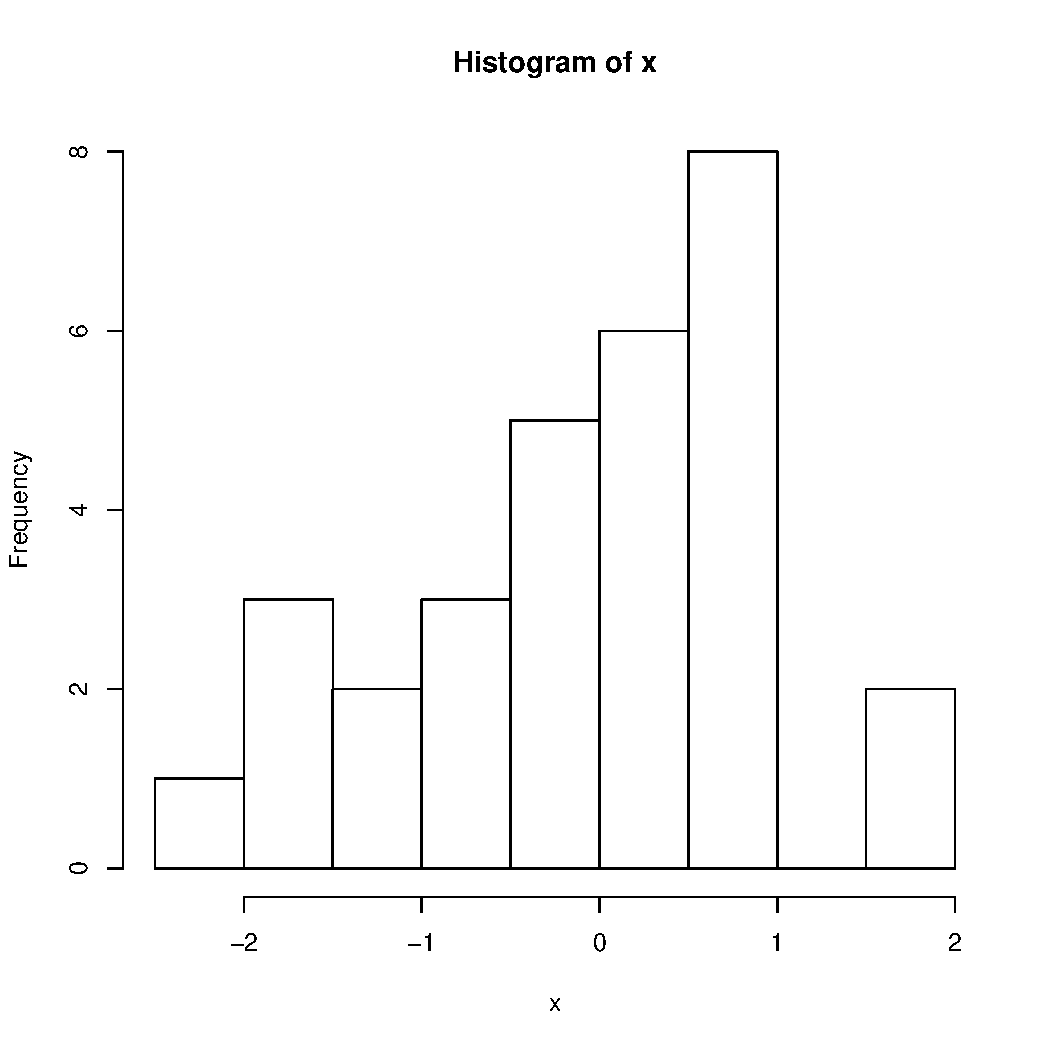
\includegraphics[width=\maxwidth]{figure/unnamed-chunk-2-1} 

\end{knitrout}

\end{document}
